\documentclass[12pt,a4paper]{article}
\usepackage[margin=1.32in]{geometry} 
\usepackage[utf8]{inputenc}
\usepackage[english]{babel}
\usepackage{amsmath}
\usepackage{amsfonts}
\usepackage{amssymb}
\usepackage{graphicx}
\usepackage{subfigure}
\usepackage{csquotes}
\usepackage{float}
\usepackage{hyperref}

\title{Prediction of Sales using Ensemble of Regressors
	\footnote{The competition was worked on as a project for \href{https://eee.uci.edu/15f/35370}{CS 273A: Machine Learning, Fall 2015}, taught by \href{http://emj.ics.uci.edu/}{Prof. Eric Mjolsness}.}
}

\author{
Karthik Prasad\and Phani Shekhar\and Rishabh Shah\and Sushruth Gopal
\vspace{2mm}
\footnote{Karthik Rajendra Prasad: Student\# 42686317, Phani Shekhar Mantripragada: Student\# 85686586, Rishabh Amit Shah: Student\# 79403075, Sushruth Mallipatna Gopal: Student\# 57803787}\\
  University of California Irvine\\
  \texttt{\{prasadkr,pmantrip,rishabas,smallipa\}@uci.edu}
}
\date{}


\begin{document}
\maketitle

\begin{abstract}
	\noindent
	Linear regression is a statistical approach for modeling relationships between a scalar dependent variable \texttt{y} and explanatory variables \texttt{X}. In this report, we present our experiments and approaches with different regression techniques in order to predict the sales of Rossmann Stores in Europe. By analyzing the data and features, we were able to draw helpful insights to train our models better. We studied and tried multiple linear regression modules, ranging from a Linear regression using Stochastic Gradient Descent to Support Vector Machines. We observed that an ensemble of bagging and boosting techniques on the transformed data patterns could better accommodate the richness in the data and the features yielding higher accuracy.
\end{abstract}

\section{Introduction}
The work presented in this report is based on one of the first \href{https://www.kaggle.com/c/rossmann-store-sales}{Kaggle competition} hosted by Rossmann Store. Kaggle, Inc. provides a platform for data mining competitions via the website \href{https://kaggle.com}{\url{https://kaggle.com}}. Companies and researchers use this platform to host  predictive modeling and analytics competitions, where data miners from all over the world compete to produce best models.
	
Rossmann\cite{RossmannWiki} is a retail company founded in 1972 by Dirk Rossmann. Currently, they operate over 3,000 drug stores in 7 European countries and are the second largest drug store chain in Germany\cite{RossmannKaggle}. Apart from Germany, they also have establishments in Poland, Hungary, Czech Republic, Albania and Turkey. This competition challenges people to predict the daily sales for a time period of 6 weeks for 1115 stores located across Germany.

Rossmann has provided the historical sales of those 1115 stores\cite{RossmannData}. The data provided by them has been organized into the following CSV files:

\begin{itemize}
	\item train.csv - Historical sales data of stores
	\item store.csv - Additional information about the stores
\end{itemize}

The data captures details such as number of customers visiting the stores, amount of sales, details of promotional offers, type of store, assortment of products sold by the store, details of the nearest competition and other related factors such as school holidays, state and public holidays. Given the above data we are supposed to predict the sales for the next 6 weeks at all stores.

\section{Previous Work}
\label{previous}

The forum on Kaggle for Rossmann Store Competition was active and posted external data \cite{externaldata} that can be used by everyone. \\ We leveraged the data mapping stores to states\cite{storeonmap} to understand the state dynamics and its effect on the sales of the store. \\ We also came across a post\cite{logtransform} (Fig. \ref{fig:logtransform}) on the forum which proved that using log transformation of the sales (instead of sales value) while calculating root-mean-squared-percentage-error(RMSPE) improves the accuracy.
\begin{figure}[!htb]
	\begin{center}
		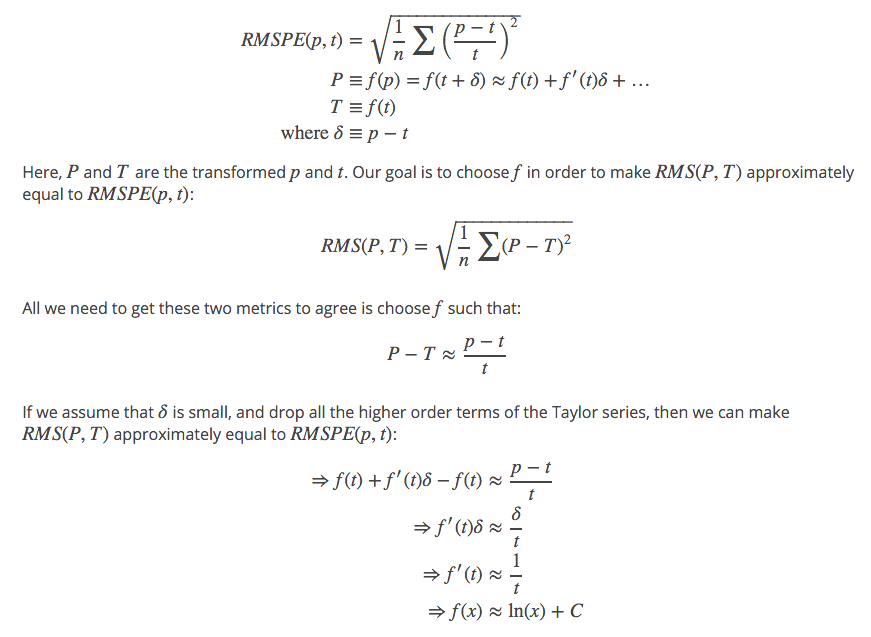
\includegraphics[scale=0.4]{images/Log_transform_for_rmspe.png}
		\caption{Relationship between between RMSPE and RMS(\texttt{log(y)})}
		\label{fig:logtransform}
	\end{center}
\end{figure}

\section{Overview and Decomposition of the Project}
We tackled the problem by trying out various techniques. We started of with simple techniques and then let the project evolve organically by incorporating the learnings at every stage.\\

Section \ref{previous} provides the information that we gathered by exploring the Kaggle forum to understand the work done by other competitors. Insightful external data and tips to start on a Kaggle project were gathered as well. This work was done by \textbf{\textit{Rishabh}}.\\
Section \ref{di} details our efforts with data analysis and building the exploratory graphs. This work was done by \textbf{\textit{Karthik}} and \textbf{\textit{Phani}} using the Pandas library\cite{pandas} in Python.\\
Section \ref{dt} expands on important data and feature engineering techniques such as One-Hot encoding, normalization, feature synthesis and mergers, outlier detection and removal, and imputing missing data. This work was done by \textbf{\textit{all four}}.\\
Section \ref{sgd} talks about Stochastic Gradient Descent on Linear Regression and the implementation details of this algorithm. This work was done by \textbf{\textit{Karthik}} and \textbf{\textit{Sushruth}} using the SGD Regressor library\cite{sgdlib} in Python.\\
Section \ref{svm} discusses Support Vector Machine and its implementation to build the prediction model for this problem. This work was done by \textbf{\textit{Rishabh}} using the Linear SVM library\cite{svrlib} in Python.\\
Section \ref{rf} highlights one of the successful techniques employed by us --  Bagging: Random Forest algorithm. The section presents our learnings from this algorithm. The feature was implemented using Random Forest Regressor Scikit Library\cite{rfr} in Python. It also presents our observations about the feature importance weight matrix and the RMSPE achieved by varying the various parameters of Random Forest Algorithm. This work was done by \textbf{\textit{Rishabh}} and \textbf{\textit{Karthik}}.\\
Section \ref{gb} presents yet another successful technique -- Gradient Boosting Algorithm and describes the implementation of this algorithm using XGBoost library\cite{github_xgb} in Python. It lists the important features and RMSPE result achieved by changing the parameters of Gradient Boosting Algorithm. This work was done by \textbf{\textit{Sushruth}} and \textbf{\textit{Phani}}. \\
After considerable analysis and experimentation, we decided to proceed with the ensemble of the above two ensemble techniques. Section \ref{ens} discusses the reasons and motivations behind this approach. This part of the project was implemented by \textbf{\textit{Rishabh}}.

\section{Data Engineering}

\subsection{Data Insights}
\label{di}
\begin{figure}[H]
	\centering
	\hspace*{-0.5in}
	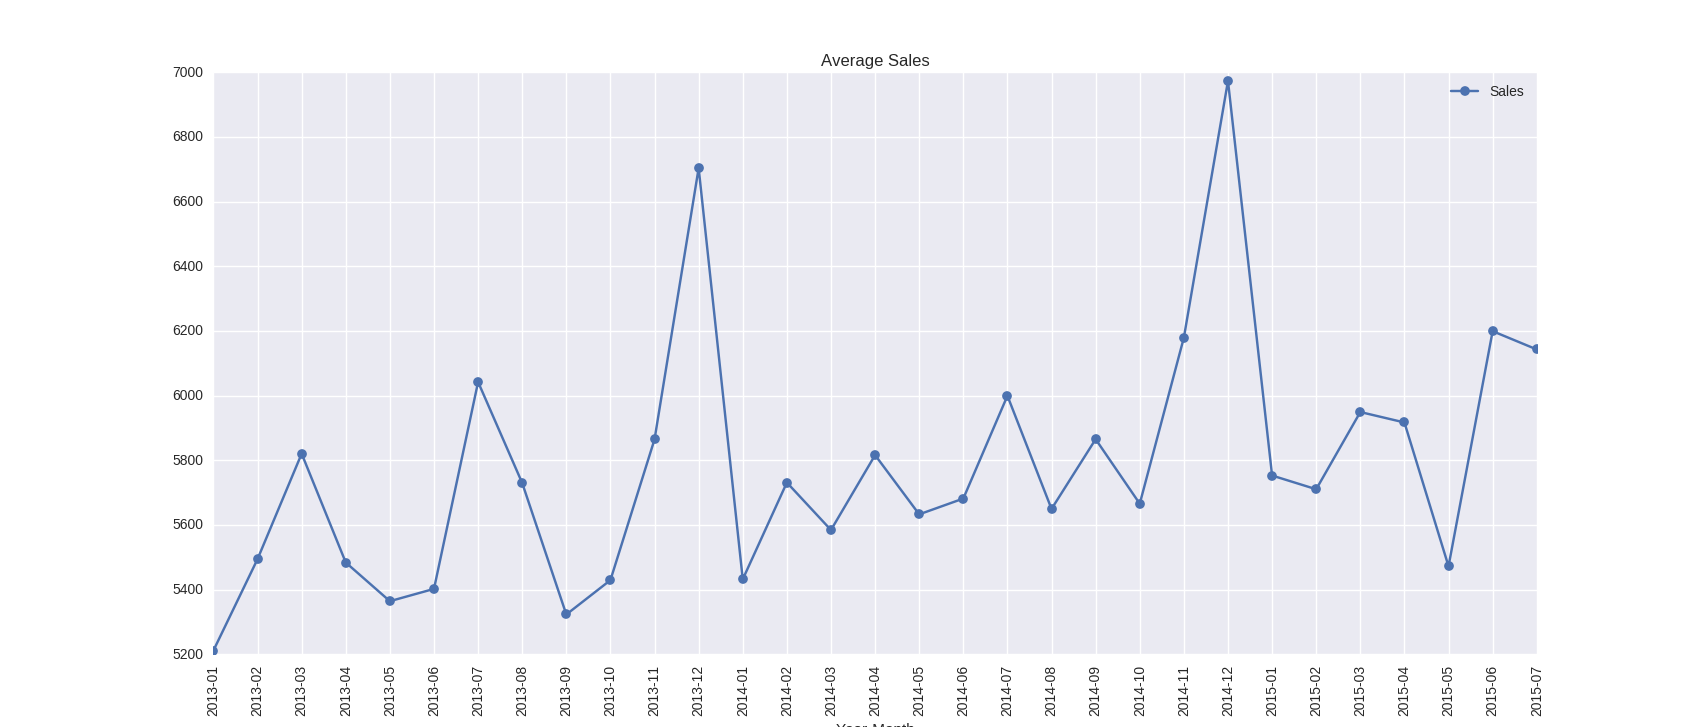
\includegraphics[width=1.25\textwidth, height=2.24in]{images/MonthWiseAvgSales.png}
	\caption{Month-wise Average Sales}
	\label{fig:mwas}
\end{figure}
    
\begin{itemize}    
	\item Plotting the average sales per month (Fig. \ref{fig:mwas}) revealed that the sales were high during the months of December, March and July; perhaps due to Christmas, Easter festivals and public holidays. 
	\item Plotting the average sales per day (Fig. \ref{fig:asbdow}) revealed that the average sales of the stores that were open on Sundays were higher than the ones that were not.
	      		    
	      \begin{figure}[H]
	      	\centering
	      	\hspace*{-0.5in}
	      	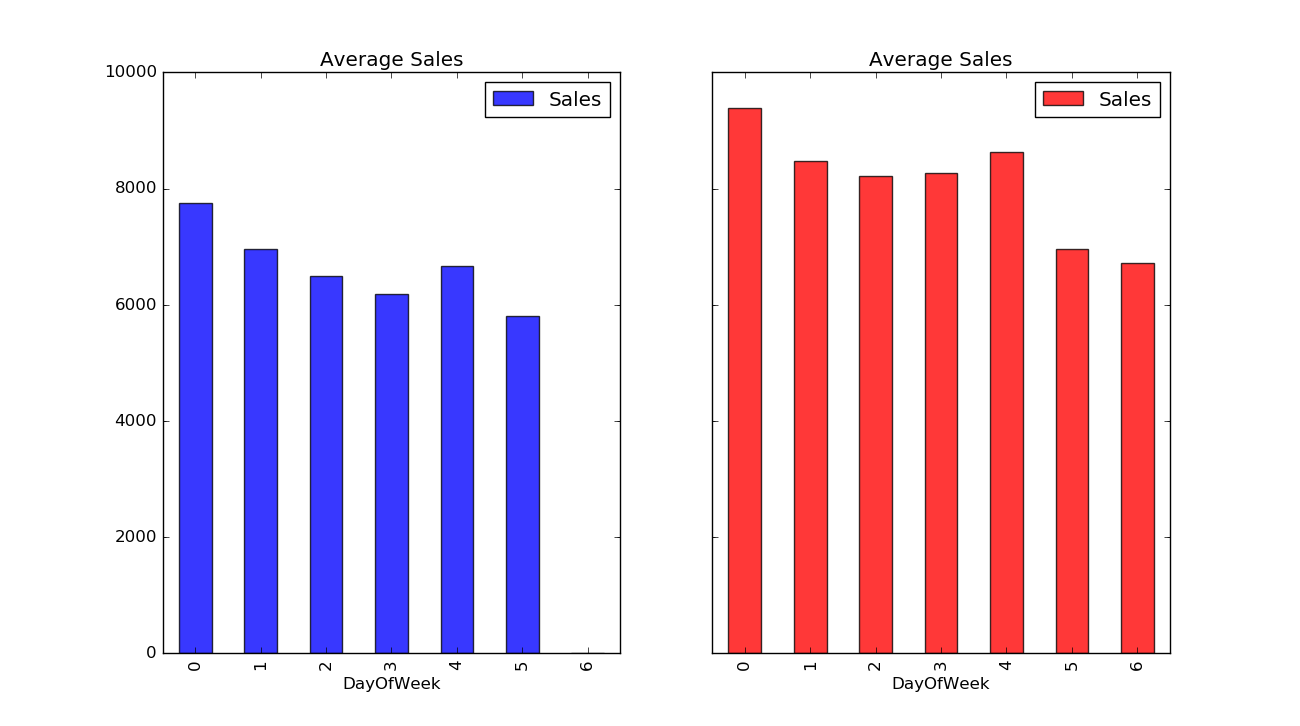
\includegraphics[width=1.25\textwidth, height=2.2in]{images/AvgSalesByDayOfWeek.png}
	      	\caption{Average Sales by Day of Week for stores closed and open on Sundays}
	      	\label{fig:asbdow}
	      \end{figure}
	          
	\item While the stores A, C, D reported the same average sales, the store type B reported much higher sales. Added to this the stores with extended assortment supplies reported larger sales. (Fig. \ref{fig:asbst} and \ref{fig:asba})
	          
	\item Promo played an important role in the sales of the store. The average sales of the stores almost doubled in the promotion weeks. Similarly, sales were higher on school holidays. (Fig. \ref{fig:asbp} and \ref{fig:asbsh})
	      		    
	      \begin{figure}[H]
	      	\centering
	      	\subfigure[Average Sales by Store Type]{
	      		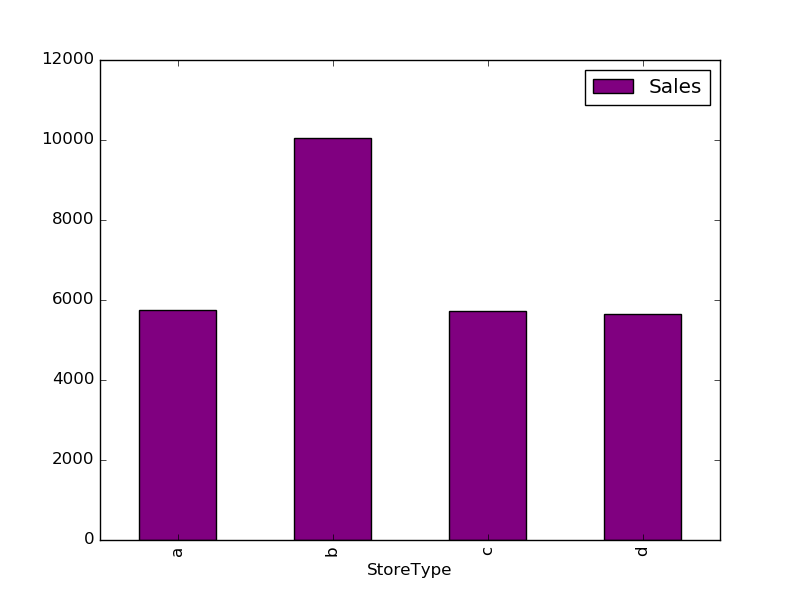
\includegraphics[width=0.42\textwidth, height=2.8in]{images/AvgSalesByStoreType.png}
	      		\label{fig:asbst}		            
	      	}				
	      	\subfigure[Average Sales by Assortment]{
	      		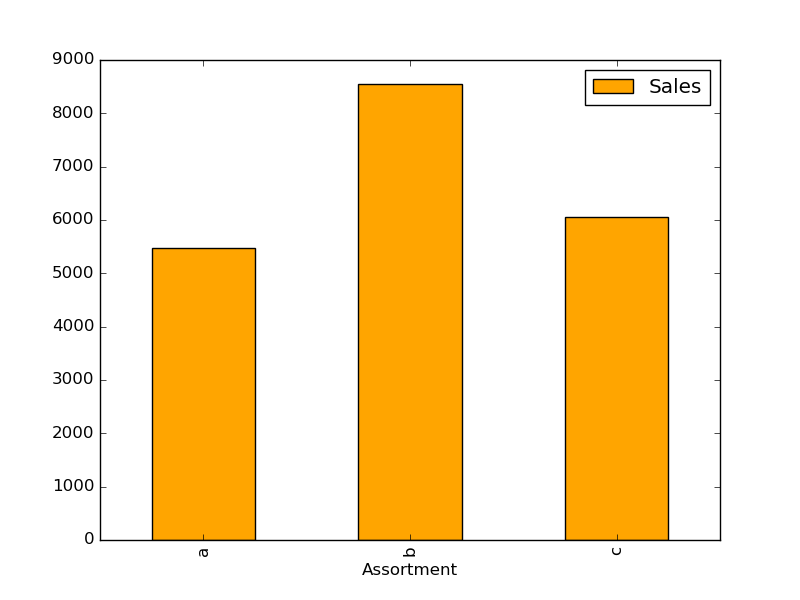
\includegraphics[width=0.42\textwidth, height=2.8in]{images/AvgSalesByAssortment.png}
	      		\label{fig:asba}
	      		}\\
	      	\subfigure[Average Sales by Promotion]{
	      		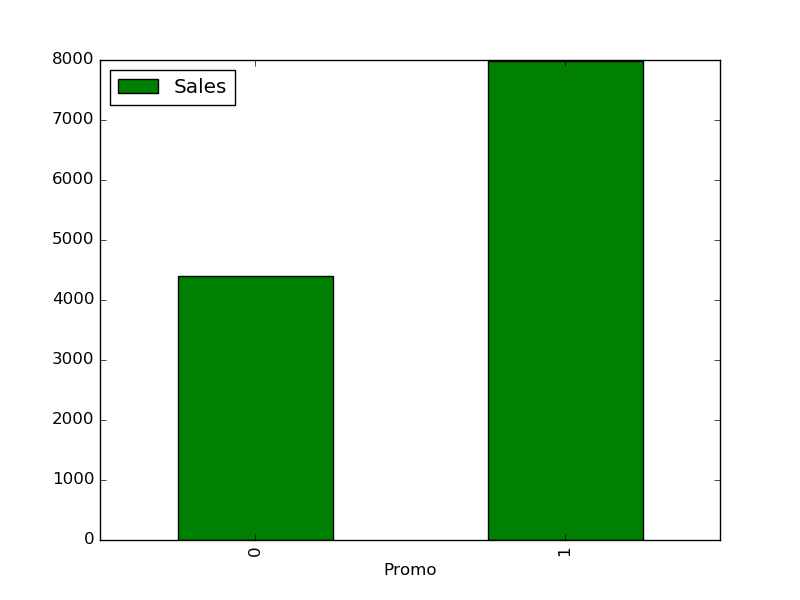
\includegraphics[width=0.42\textwidth, height=2.8in]{images/AvgSalesByPromo.png}
	      		\label{fig:asbp}
	      	}
	      	\subfigure[Average Sales by School Holiday]{
	      		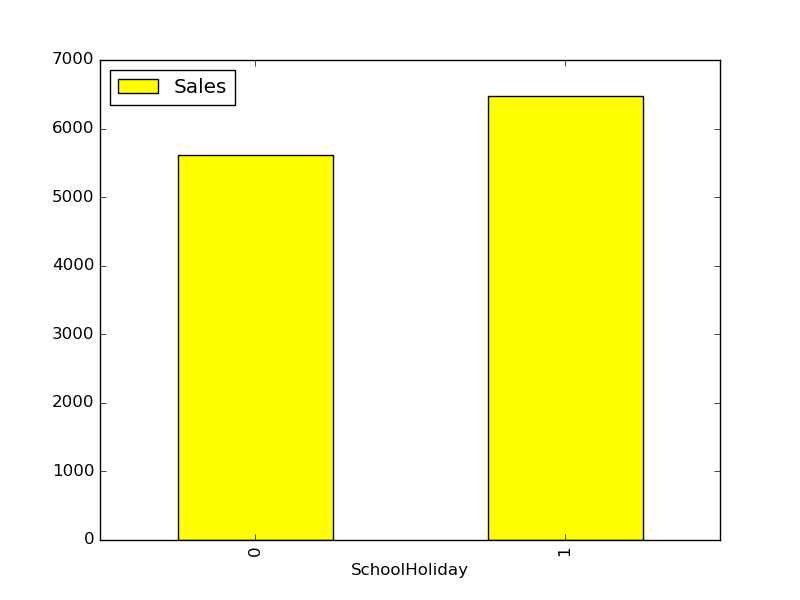
\includegraphics[width=0.42\textwidth, height=2.8in]{images/AvgSalesBySchoolHol.png}
	      		\label{fig:asbsh}
	      	}
	      	\caption{Sales by Features}
	      	\label{fig:salesbyfeatures1}        			
	      \end{figure}
	      		    
	\item Plotting the sales of stores with time exposed anomalies in the data. Sales data for some months were missing for certain stores,  whereas some stores reported spike in sales just before they were closed as shown in Fig. \ref{fig:dataanalysis1}. These sets were one time events and considered anomalies as they had a negative impact on the average sales being predicted.
	      
	\item Similarly, some stores which were open on sundays never reported zero sales. Out of the 1115 stores some were open on sundays, where as the others were not. But plotting the sales time graph(Fig. \ref{fig:dataanalysis2}) we realized that some stores were open on sundays for certain weeks and closed for other. 
	      		    
	      \begin{figure}[H]
	      	\centering
	      	\subfigure{
	      		\label{fig:d1}
	      		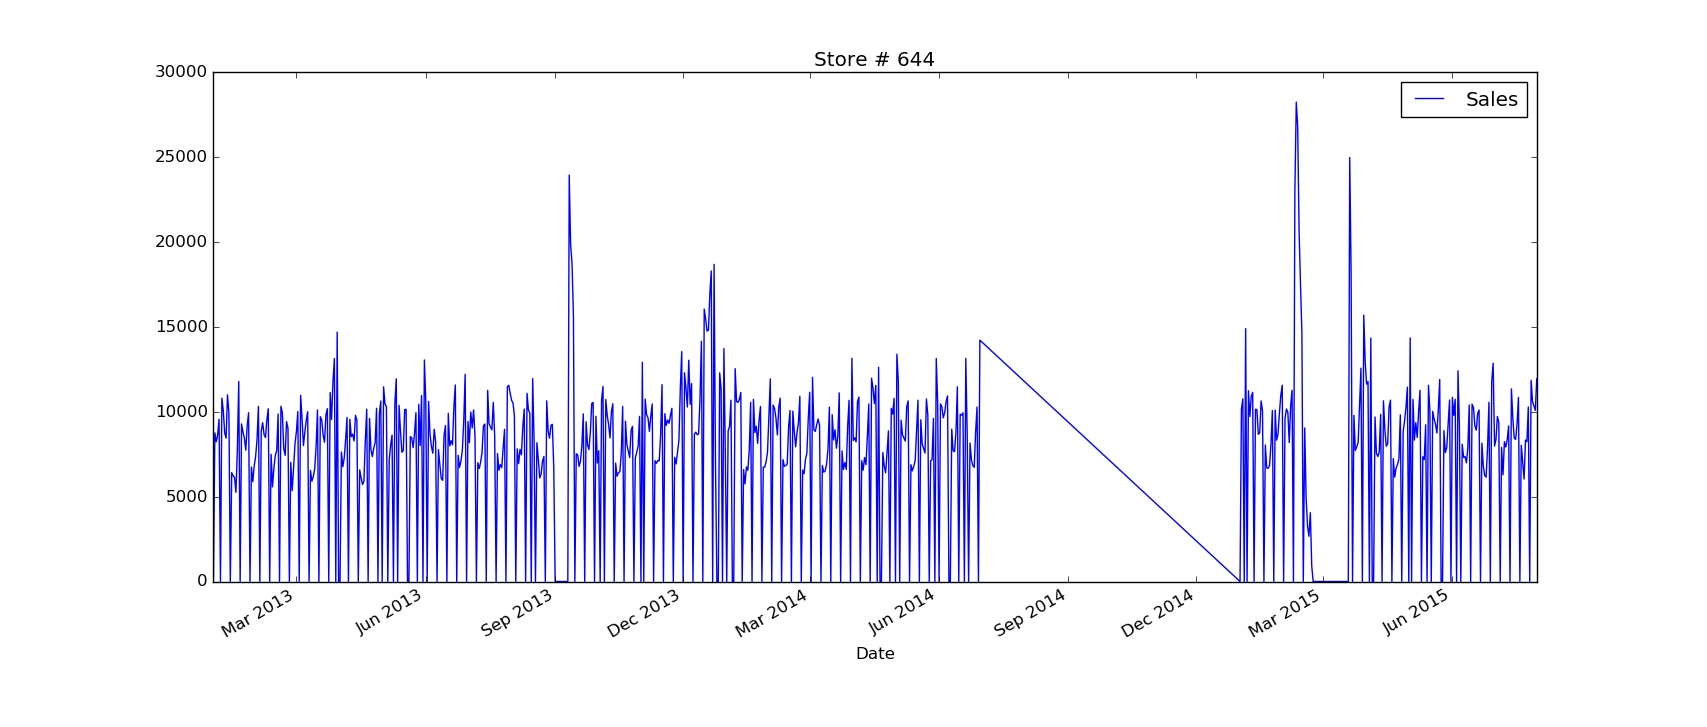
\includegraphics[width=1\textwidth, height=2.25in]{images/1.png}
	      		}\\
	      	\vspace{-0.17in}
	      	\subfigure{
	      		\label{fig:d2}
	      		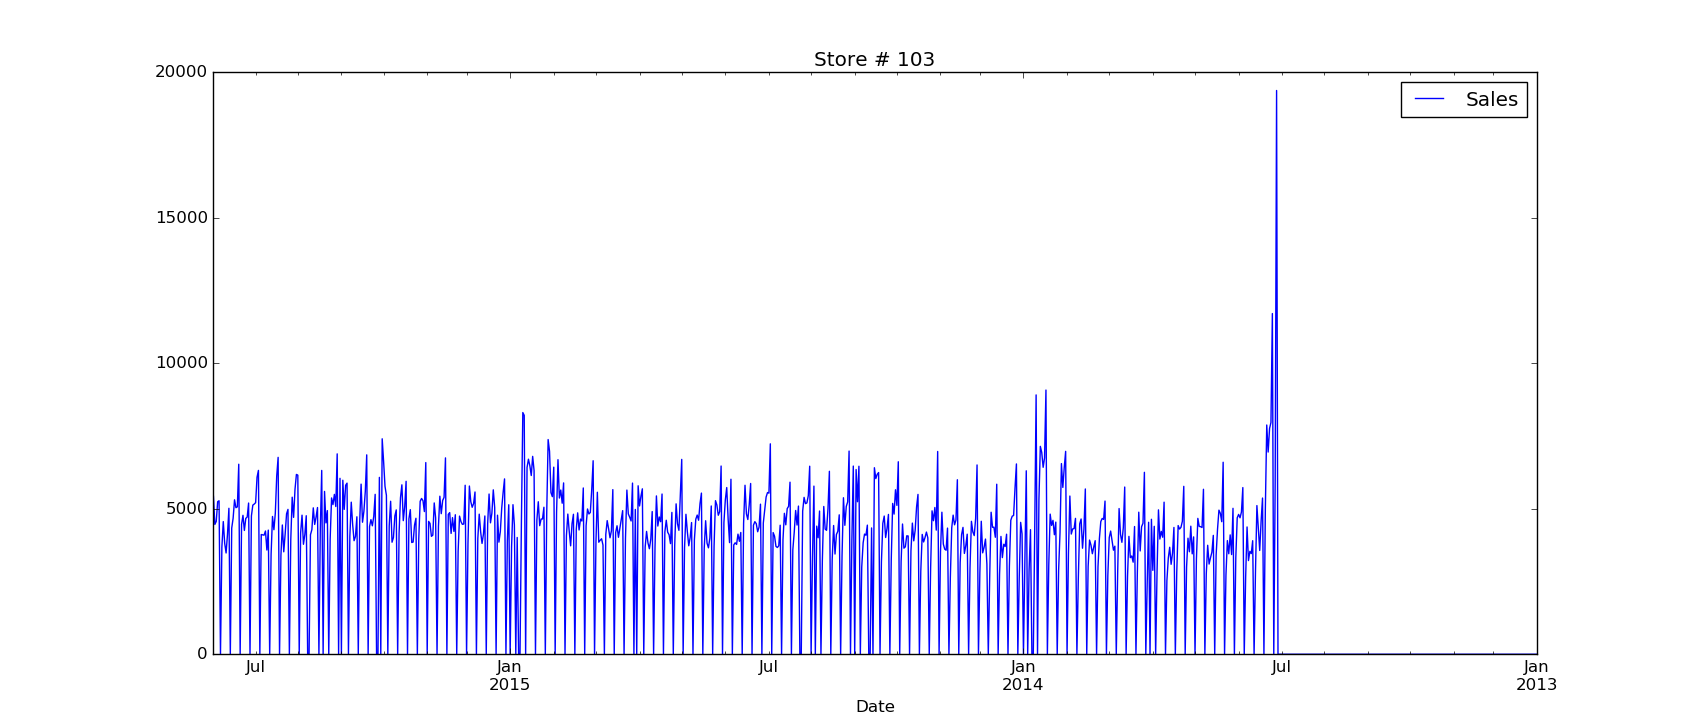
\includegraphics[width=1\textwidth, height=2.2in]{images/2.png}
	      		}\\
	      	\vspace{-0.17in}
	      	\subfigure{
	      		\label{fig:d3}
	      		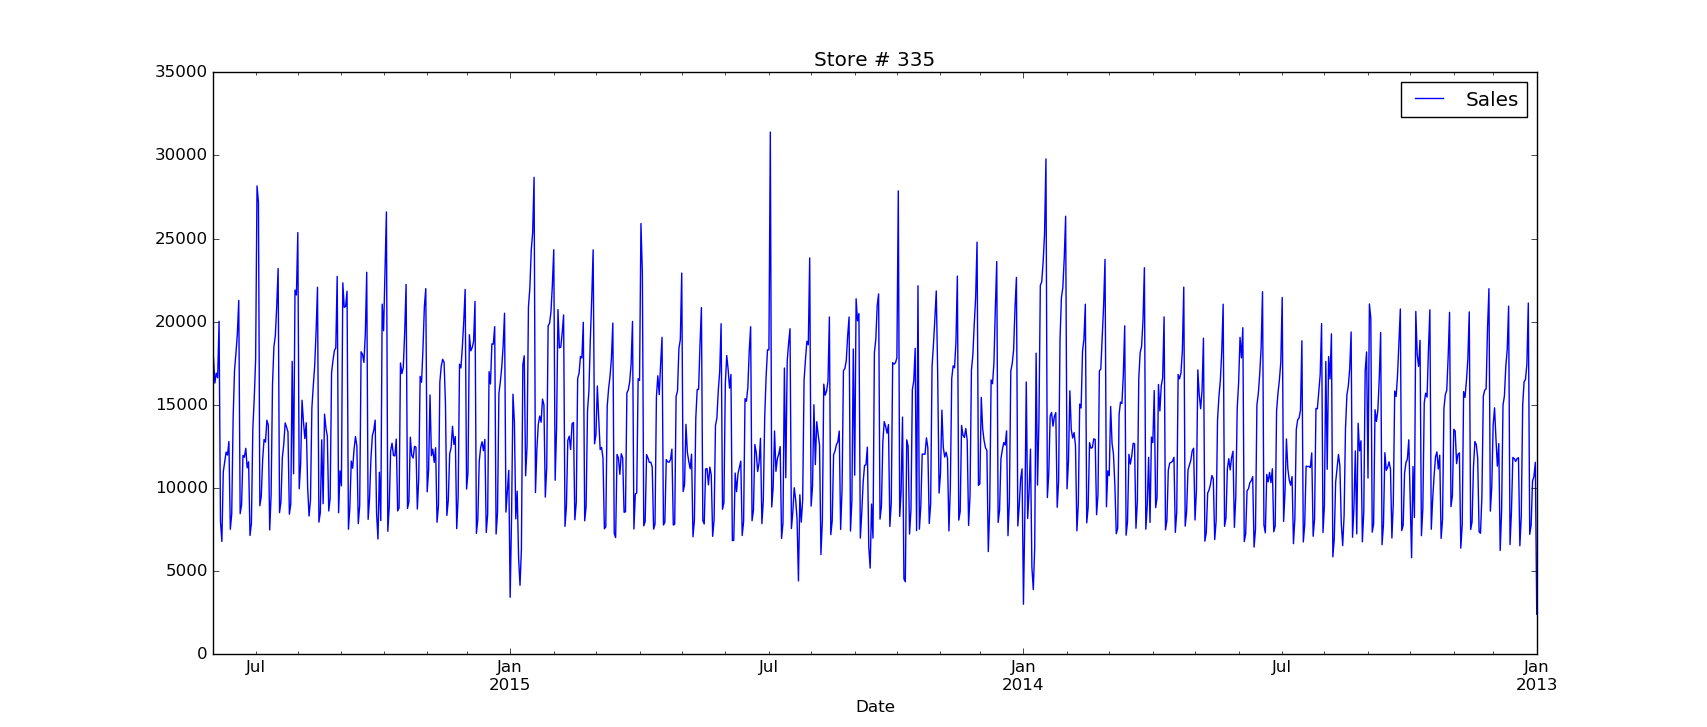
\includegraphics[width=1\textwidth, height=2.2in]{images/3.png}
	      	}
	      	\caption{Interesting Data Patterns (Sales per store v/s Time)}
	      	\label{fig:dataanalysis1}
	      \end{figure}
	           
	      \begin{figure}[H]
	      	\centering
	      	\subfigure{
	      		\label{fig:d4}
	      		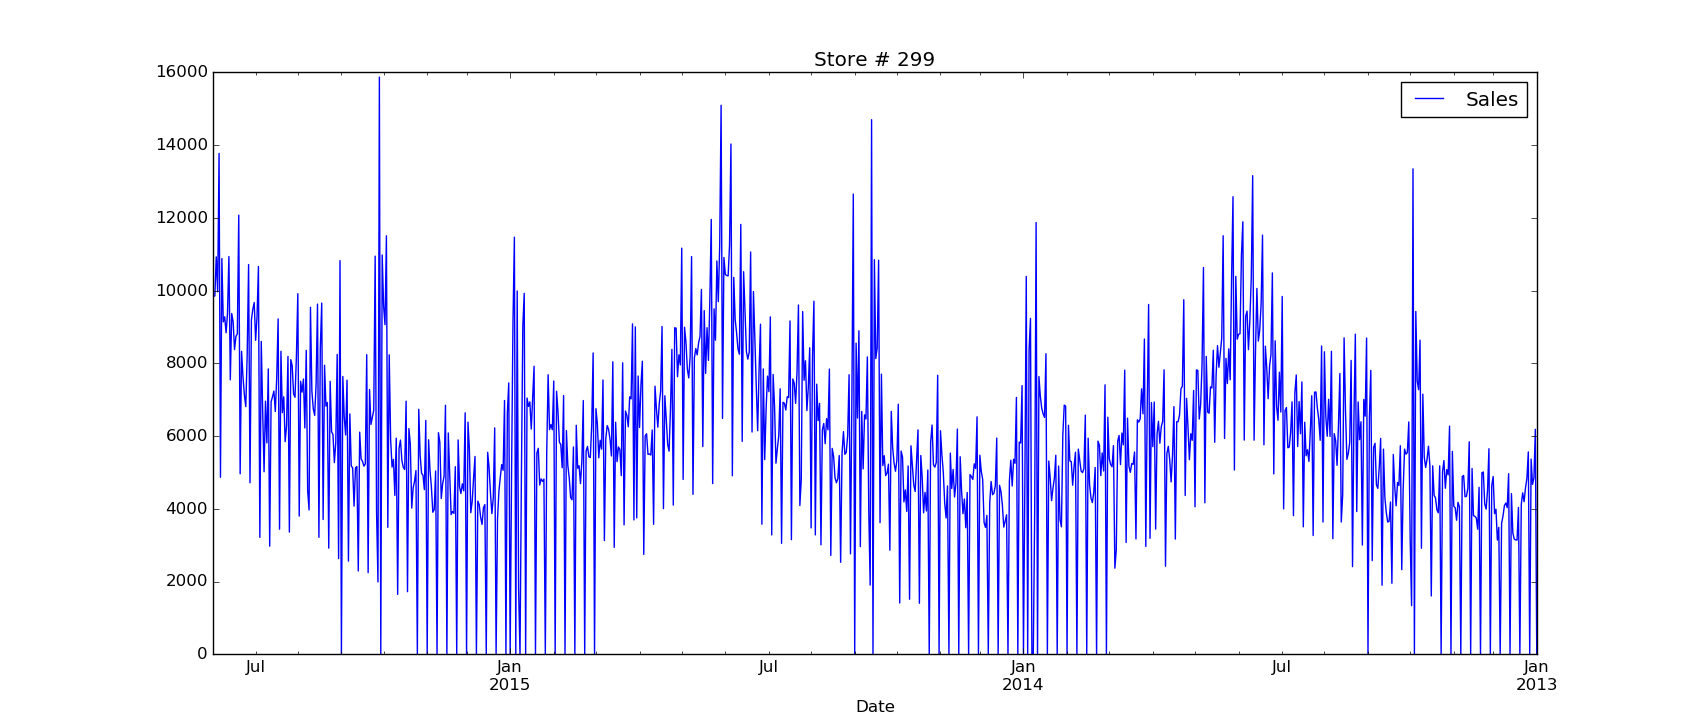
\includegraphics[width=1\textwidth, height=2.2in]{images/4.png}
	      	}
	      	\caption{Interesting Data Patterns (Sales per store v/s Time)}
	      	\label{fig:dataanalysis2}		
	      \end{figure}
	      		    
\end{itemize}
    
    
    
    
\subsection{Data Transformation}
\label{dt}
\begin{itemize}
	
	\item \textbf{One Hot Encoding}: Many categorical variables were provided in the raw feature list such as - DayOfWeek, StoreType, Assortment, MonthOfYear. By one-hot encoding, we bloated the feature space as DayOfWeek got converted to 6 features (Sunday represented as all zeroes). This resulted in RMSPE score improvement by 0.15.
	      
	\item \textbf{Removing data outliers}: Unexpectedly high sales (four times the mean value) were reported on few days for limited stores. These outliers and anomalies were clipped and limited to mean $ \pm $ 3*standard deviation
	      
	\item \textbf{Addition of New features}: Stores open on sundays throughout the year reported higher average sales than the other stores which were closed on sundays. A new feature was added to report such stores. Also, promo interval was introduced by merging few features from the training set.
	      
	\item \textbf{Imputation of Missing Data}: Few stores were closed for more than six months due to refurbishment. This data was affecting the final model and had to be excluded from the final training set. 
	      
	\item \textbf{Normalizing and Data Binning}: CompetitionDistance and CompetitionOpen had a high cardinality in their data and ranged from 0 to 35000. This had to be normalized and binned to reduce its effect on sales.
\end{itemize}
\section{Implementation}
\subsection{Linear Regression Model with Stochastic Gradient Descent}
\label{sgd}
Our approach to predict the sales from the given set of features was to first check the efficiency achieved using a simple linear regression model. As we had more than a million entries to train on, we used Stochastic Gradient Descent\cite{sgdlib} with the simple regression model on this large data set. We experimented with different error functions, learning rate and number of iterations. The best result was attained with the Huber loss function\cite{wiki_hu}, 1000 iterations and a learning rate of 0.01. The RMSPE was around \textit{0.4271}. From this experiment it was evident that the simple linear regressor would not be able to capture all the patterns in the data, and we needed a better regression model.

\subsection{Support Vector Machines}
\label{svm}
A linear regression model was not able to fit the data points accurately. We decided to use Support Vector Regression to project the data to a higher dimensional space using a kernel where we could perform linear curve fitting. We implemented this algorithm using the SVR Library\cite{svrlib} in Python with Linear, polynomial of degree 4, Radial Basis Function kernels\cite{kernel} and epsilon insensitive loss function\cite{bishop}. Training the data with the entire sample set was computationally expensive, O(Number of features * Training samples\textsuperscript{2})\cite{svmruntime}. Training the model using smaller chunks of 20000 samples (out of one million data points) did not yield good results(RMSPE \textgreater  \ 10).

\subsection{Bagging - Random Forest Algorithm}
\label{rf}
Bagging involves training multiple models using bootstrap data sets and aggregating the result of the individual models\cite{bishop}. We used a particular type of Bagging technique called Random Forest. Random Forest\cite{wiki_rf} constructs a collection of decision trees\cite{wiki_dt} during training phase and outputs the mean prediction of the individual trees. A random set of features are used to train the decision tree over random training data samples. This is done to make sure the individual models are not correlated.

Random Forest is trained on the data and the performance of the algorithm is recorded by varying the number of trees used. Cross validation error is used to record the performance.
\begin{figure}[!htb]
	\centering
	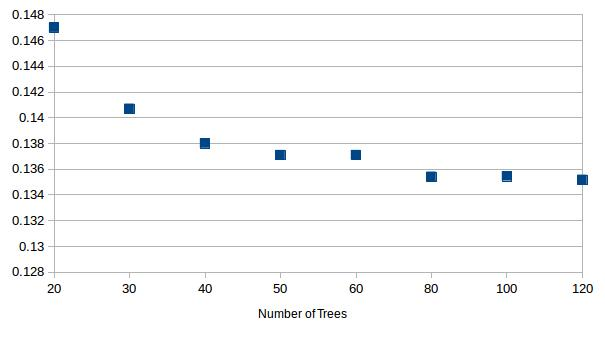
\includegraphics[width=0.8\textwidth, height=2.5in]{images/RF_Error_Plot.jpg}
	\caption{RMSPE v/s No. of Trees}
	\label{fig:rfres}
\end{figure}

As evident from the results (Fig. \ref{fig:rfres}), the performance of the algorithm saturates after the number of trees is around 100 which is used to calculate the error on the test data on the Kaggle Competition.
Random Forests are biased in favor of categorical variables with different number of levels while calculating the feature importance\cite{wiki_rf}. One-hot encoding described in Section Data Transformation  helped us overcome this problem. The feature importance as ranked by the Random Forest is as shown in Fig. \ref{fig:rfimp}

\begin{figure}[H]
	\centering
	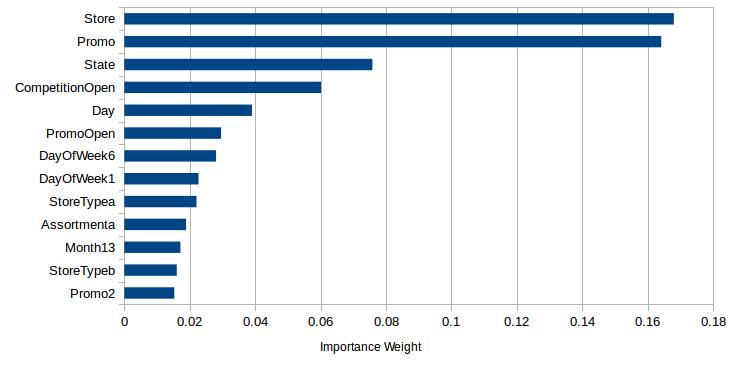
\includegraphics[width=0.8\textwidth, height=2.5in]{images/RF_Feature_Importance.jpg}
	\caption{Feature importance as determined by Random Forest}
	\label{fig:rfimp}
\end{figure}

\subsection{Gradient Boosting Algorithm}
\label{gb}
Boosting involves training multiple models in sequence in which the error function used to train a particular model depends on the performance of previous models.\cite{bishop} Gradient Boosting\cite{wiki_bo} is a technique which constructs a collection of decision trees during training phase and outputs the weighted average of prediction of the individual trees.
Gradient Boosting is known to perform better than Random Forest in the case of correlated features\cite{boost}. The performance of the algorithm is recorded by varying the number of boosting iterations.
\\
\\
As indicated by the results (Fig. \ref{fig:gbres}), 800 iterations are used to calculate the error on the test data. The feature importance as ranked by the Boosting algorithm is as shown in Fig. \ref{fig:gbimp}
\begin{figure}[H]
	\centering
	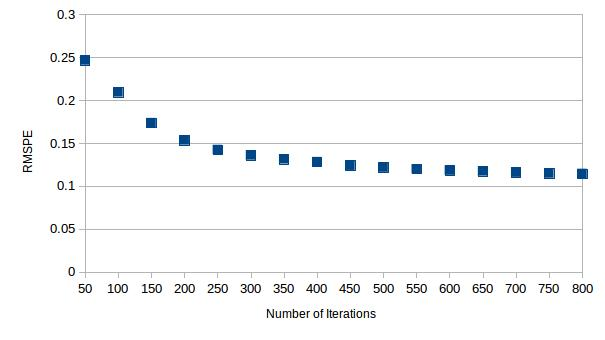
\includegraphics[width=0.8\textwidth,height=2.5in]{images/Boost_Error_Plot.jpg}
	\caption{RMSPE v/s No. of iterations}
	\label{fig:gbres}
\end{figure}

\begin{figure}[H]
	\centering
	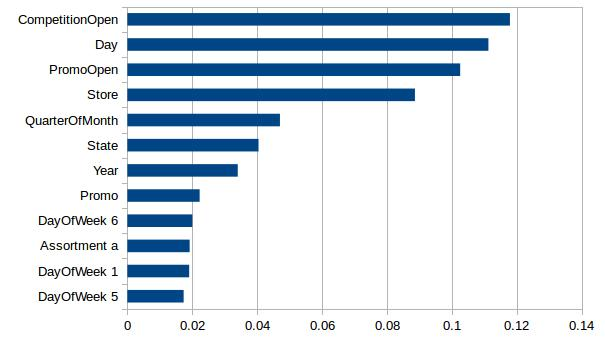
\includegraphics[width=0.8\textwidth, height=2.5in]{images/Boost_Feature_Importance.jpg}
	\caption{Feature importance as determined by Gradient Boosting}
	\label{fig:gbimp}
\end{figure}

\subsection{Ensemble of Ensembles}
\label{ens}
The Gradient boosting technique yielded slightly better accuracy than the Random Forest algorithm. However, boosting has a tendency to over-fit the training data\cite{wiki_rf}\cite{wiki_bo}. Therefore, we tried to use weighted average of the predictions made by the two models by giving higher weight to the better model (boosting) and obtained improved results (Table \ref{tbl:results}). 

\begin{table}[H]
	\centering
	\resizebox{0.88\textwidth}{1cm}{
		\begin{tabular}{ l | c c c | l}
			                         & SGD on Linear Regression & Gradient Boosting & Random Forest & Ensemble of Ensembles \\ \hline
			\textbf{Raw Data}        & 0.5483                   & 0.1348            & 0.1536        &                       \\
			\textbf{Engineered Data} & 0.4271                   & 0.1190            & 0.1328        & \large\textbf{0.1179} 
		\end{tabular}
	}
	\caption{RMSPE rates for different algorithms and data combinations}
	\label{tbl:results}
\end{table}

\section{Future Work}
The current set of features provided a strong model to play with and we were successful to an extent to get the best out of them. Nevertheless, addition of more features that could potentially influence the predictions are to be considered. The information about weather, for instance, can play a vital role in determining the customers' willingness to visit the store which is directly related to sales. Similarly, clustering the stores based on the geographical regions and modeling each region separately might help in improving the accuracy. Since the stores  are located in majorly Germany, the local events such as festivals, football matches can heavily influence the sales figures. Most importantly, given time-series nature of data, we strongly feel that running time-series modeling techniques such as ARIMA\cite{arima} can significantly boost our accuracy.

\section{Conclusion}
The project helped in solidifying our understanding of the different machine learning techniques and algorithms. We started by directly applying machine learning algorithms on raw data and then organically evolved by polishing the data and using robust algorithms. The exercise emphasized the importance of data analysis and data engineering before running the algorithms on them. We learnt that each technique and model comes with its own set of advantages and disadvantages and no one model can accommodate the data. Accordingly, after the initial attempts of running various algorithms such as Support Vector Machines and SGD on Linear Regression, we obtained better results with ensemble regression techniques: boosting(Gradient Boosting) and bagging(Random Forest). Further, to prevent over-fitting and be robust to correlated features, we used a weighted average of the above techniques and obtained even better results.

\begin{thebibliography}{9}
	
	\bibitem{bishop}
	Bishop, Christopher M. \textit{Pattern Recognition and Machine Learning}. New York: Springer, 2006. Print.
	
	\bibitem{RossmannWiki}
	\enquote{\textit{Wikipedia}. (Rossmann Company), n.d. Web. 09 Dec. 2015.} \textit{Web}. \href{https://en.wikipedia.org/wiki/Rossmann_(company)}{\url{https://en.wikipedia.org/wiki/Rossmann_(company)}}
	
	\bibitem{RossmannKaggle}
	\enquote{Rossmann Store Sales} \textit{Description}. N.p., n.d. Web. 09 Dec. 2015. \textit{Web}. \href{https://www.kaggle.com/c/rossmann-store-sales}{\url{https://www.kaggle.com/c/rossmann-store-sales}}
	
	\bibitem{RossmannData}
	\enquote{Rossmann Store Sales} Data. \textit{Web}. \href{https://www.kaggle.com/c/rossmann-store-sales/data}{\url{https://www.kaggle.com/c/rossmann-store-sales/data}}
	
	\bibitem{externaldata}
	\enquote{Rossmann Store Sales} External Data and Other Information. \textit{Web}. \href{https://www.kaggle.com/c/rossmann-store-sales/forums/t/17229/external-data-and-other-information.}{\url{https://www.kaggle.com/c/rossmann-store-sales/forums/t/17229/external-data-and-other-information.
	}}
	
	\bibitem{storeonmap}
	\enquote{Rossmann Store Sales}. Putting Stores on the Map. \textit{Web}. \href{https://www.kaggle.com/c/rossmann-store-sales/forums/t/17048/putting-stores-on-the-map.}{\url{https://www.kaggle.com/c/rossmann-store-sales/forums/t/17048/putting-stores-on-the-map.}}
	
	\bibitem{logtransform}
	\enquote{Rossmann Store Sales}. Connection between RMSPE and the log transform. \textit{Web}. \href{https://www.kaggle.com/c/rossmann-store-sales/forums/t/17026/a-connection-between-rmspe-and-the-log-transform.}{\url{https://www.kaggle.com/c/rossmann-store-sales/forums/t/17026/a-connection-between-rmspe-and-the-log-transform.}}
	
	\bibitem{pandas}
	\enquote{Python Data Analysis Library}. N.p., n.d. Web. 
	\href{http://pandas.pydata.org/}{\url{http://pandas.pydata.org/}}
	
	\bibitem{python}
	\enquote{Welcome to Python.org.} Python. N.p., n.d. Web. 9 Dec. 2015. 
	\href{https://www.python.org/}{\url{https://www.python.org/}}
	
	\bibitem{svrlib}
	\enquote{Sklearn svm LinearSVR} \textit{Linear SVR}. N.p., n.d. Web. 9 Dec. 2015. \href{http://scikit-learn.org/stable/modules/generated/sklearn.svm.LinearSVR.html\#sklearn.svm.LinearSVR}{\url{http://scikit-learn.org/stable/modules/generated/sklearn.svm.LinearSVR.html\#sklearn.svm.LinearSVR}}
	
	\bibitem{sgdlib}
	\enquote{Sklearn linear\_model SGDRegressor} \textit{SGD Regressor}. N.p., n.d. Web. 9 Dec. 2015. \href{http://scikit-learn.org/stable/modules/generated/sklearn.linear_model.SGDRegressor.html}{\url{http://scikit-learn.org/stable/modules/generated/sklearn.linear_model.SGDRegressor.html}}
	
	\bibitem{rfr}
	\enquote{Sklearn.ensemble.RandomForestRegressor} \textit{Random Forest Regressor}. N.p., n.d. Web. 9 Dec. 2015. \href{http://scikit-learn.org/stable/modules/generated/sklearn.ensemble.RandomForestRegressor.html}{\url{http://scikit-learn.org/stable/modules/generated/sklearn.ensemble.RandomForestRegressor.html}}
	
	\bibitem{kernel}
	\enquote{Kernel Approximation} \textit{Radial Basis Function Kernel}. N.p., n.d. Web. 9 Dec. 2015. \href{http://scikit-learn.org/stable/modules/kernel_approximation.html\#radial-basis-function-kernel}{\url{http://scikit-learn.org/stable/modules/kernel_approximation.html\#radial-basis-function-kernel}}
	
	
	\bibitem{github_xgb}
	\enquote{Dmlc/xgboost} \textit{GitHub - XGBoost} N.p., n.d. Web. 9 Dec. 2015. \href{https://github.com/dmlc/xgboost}{\url{https://github.com/dmlc/xgboost}}
	
	\bibitem{svmruntime}
	Chapelle, Olivier. \enquote{Training a Support Vector Machine in the Primal.} \textit{Neural Computation} 19.5 (2007): 1155-178. Web.
	\href{http://www.kyb.mpg.de/fileadmin/user_upload/files/publications/attachments/neco_\%5b0\%5d.pdf}{\url{http://www.kyb.mpg.de/fileadmin/user_upload/files/publications/attachments/neco_\%5b0\%5d.pdf}}
	
	\bibitem{wiki_hu}
	\enquote{Wikipedia. Wikimedia Foundation}, Huber Loss n.d. Web. 09 Dec. 2015. \href{https://en.wikipedia.org/wiki/Huber_loss}{\url{https://en.wikipedia.org/wiki/Huber_loss}}
	
	\bibitem{wiki_rf}
	\enquote{Wikipedia. Wikimedia Foundation}, Random Forest n.d. Web. 09 Dec. 2015. \href{https://en.wikipedia.org/wiki/Random_forest}{\url{https://en.wikipedia.org/wiki/Random_forest}}
	
	\bibitem{wiki_bo}
	\enquote{Wikipedia. Wikimedia Foundation}, Gradient Boosting n.d. Web. 09 Dec. 2015. \href{https://en.wikipedia.org/wiki/Gradient_boosting}{\url{https://en.wikipedia.org/wiki/Gradient_boosting}}
	
	\bibitem{wiki_dt}
	\enquote{Wikipedia. Wikimedia Foundation}, Decision Tree Learning n.d. Web. 09 Dec. 2015. \href{https://en.wikipedia.org/wiki/Decision_tree_learning}{\url{https://en.wikipedia.org/wiki/Decision_tree_learning}}
	
	\bibitem{boost}
	\enquote{Dmlc/xgboost} \textit {GitHub} N.p., n.d. Web. 09 Dec. 2015. \href{https://github.com/dmlc/xgboost/blob/master/R-package/vignettes/discoverYourData.Rmd}{\url{https://github.com/dmlc/xgboost/blob/master/R-package/vignettes/discoverYourData.Rmd}}
	
	\bibitem{arima}
	\enquote{Autoregressive Integrated Moving Average} \textit{Wikiwand}. N.p., n.d. Web. 10 Dec. 2015.
	\href{https://www.wikiwand.com/en/Autoregressive_integrated_moving_average}{\url{https://www.wikiwand.com/en/Autoregressive_integrated_moving_average}}
	
\end{thebibliography}
\end{document}